\documentclass[]{beamer}

\usepackage[utf8]{inputenc}
\usepackage[T1]{fontenc}
\usepackage{helvet}
\usepackage[english]{babel}

\usetheme{LUH}


% format numbers
\usepackage{siunitx}
%https://tex.cloud.uni-hannover.de/project/6677e7bc8f12321099572893
\sisetup{
  locale=US,
  group-digits = integer,
  round-mode = places,
  round-precision = 3,
  round-pad = false,
  mode = match % the numbers are printed in text or math mode matching their surrounding
}
% better itemize and enumerate
\usepackage{enumitem}
\setlist[itemize]{label=--} 
\setlist[enumerate]{label=\arabic*.} 
% \setlist[enumerate,1]{label=\alph*)}
% enables \enquote command for better quotation
\usepackage[nolist,nohyperlinks]{acronym}
\usepackage{csquotes}
\usepackage{ragged2e}

\usepackage{booktabs}
\usepackage[table]{xcolor}

\usepackage{tikz}
\usetikzlibrary{arrows, shapes, positioning, calc}

\usepackage[
  backend=biber,
  natbib=true,
  citestyle=authoryear,
  maxcitenames=1,
  maxbibnames=5,
]{biblatex}
\bibliography{literature.bib}
\renewcommand*{\bibfont}{\normalfont\scriptsize}

\usepackage{hyperref}
\hypersetup{
  pdftitle={Developing Interpretable Style Vectors to Steer Large Language Models towards Group-Specific Explanation Generation},
  pdfsubject={Master's Thesis Presentation},
  pdfauthor={Janek Prange}
  plainpages=false,           %   -
  colorlinks=false,           %   - colorize links?
  pdfborder={0 0 0},          %   -
  breaklinks=true,            %   - allow line break inside links
  bookmarksnumbered=true,     %
  bookmarksopen=true,          %
  pdfpagemode=UseNone,
}

\title[Master's Thesis Presentation]{Developing Interpretable Style Vectors to Steer Large Language Models towards Group-Specific Explanation Generation}
\date{08.04.2025}
% \date[08.04.2025]{08.04.2025}
\author{Janek Prange}
\unilogo{
\includegraphics[height=\LUHLogoHeight]{img/luh-logo.png}}
\logo{
\includegraphics[height=\LUHLogoHeight]{img/luh_ai-logo.png}}
\titleimage{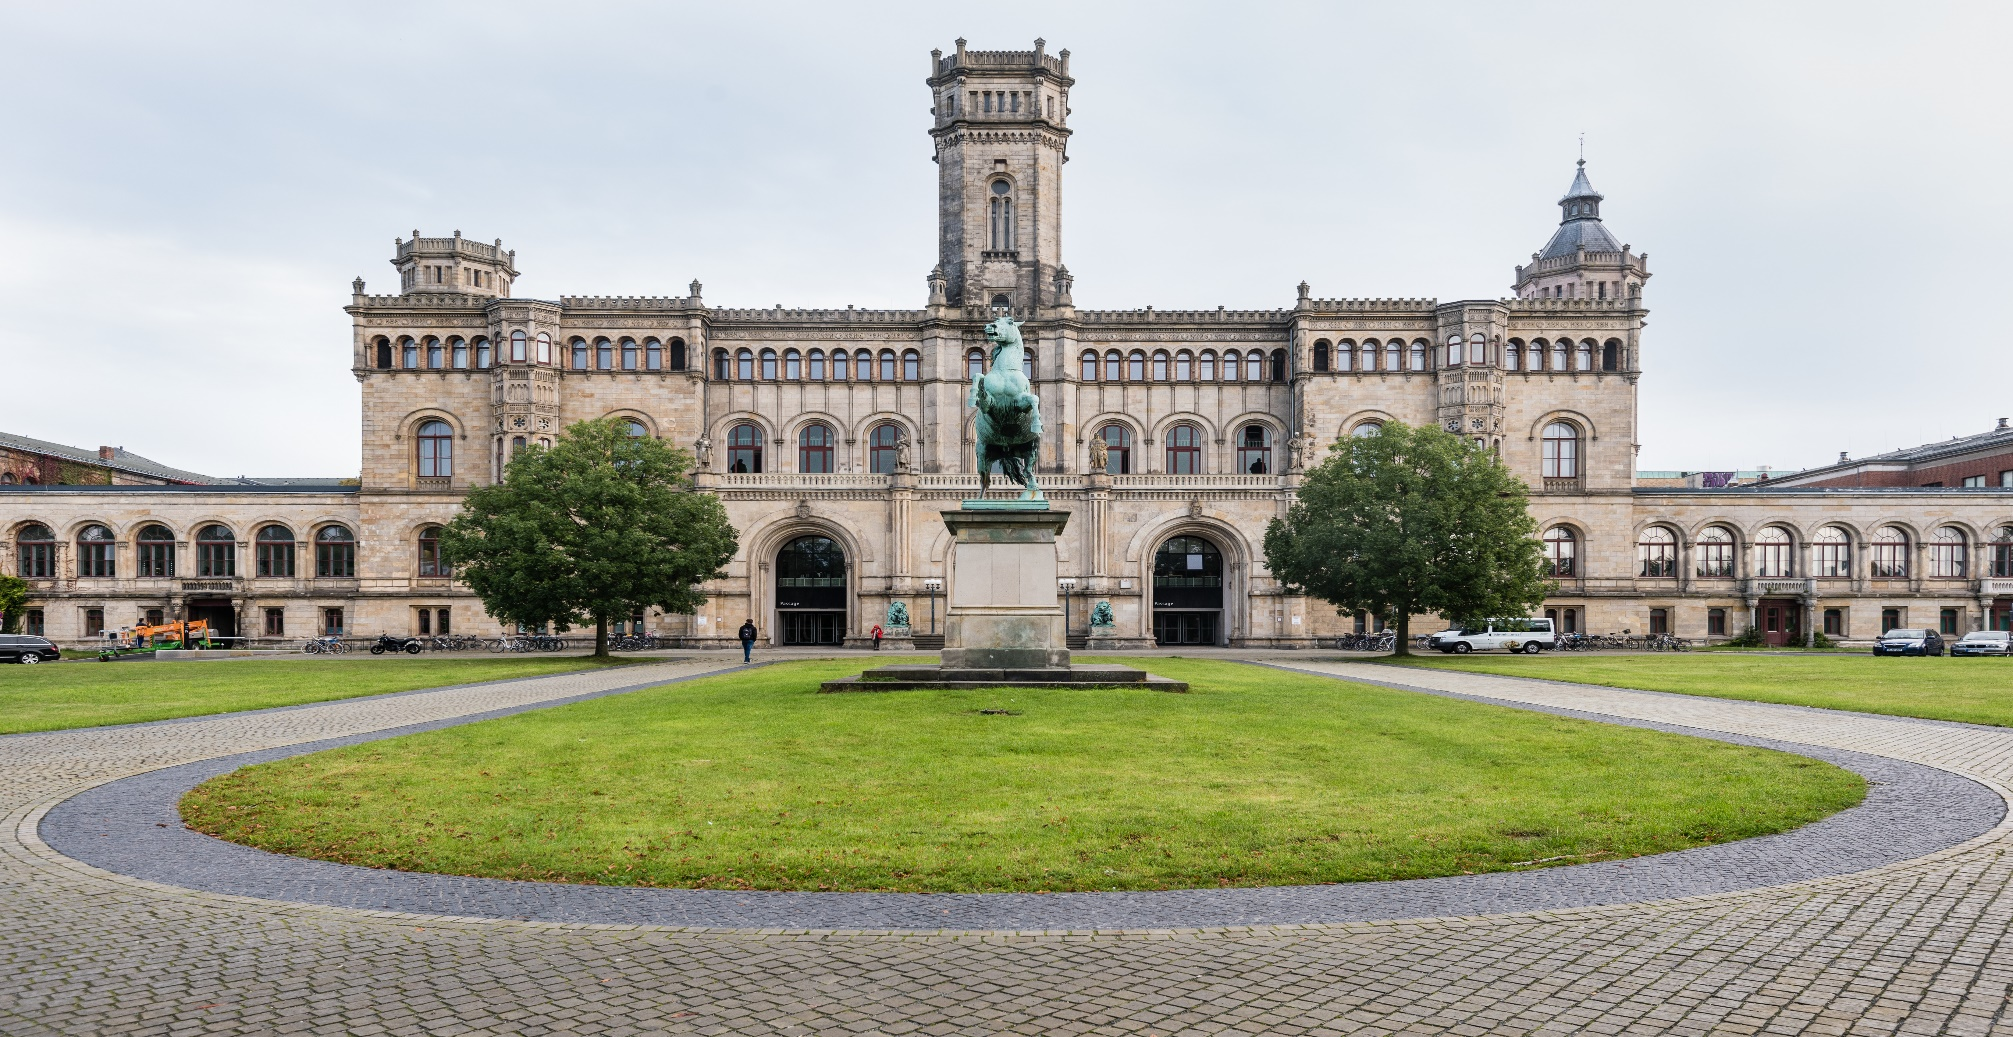
\includegraphics[width=.7\paperwidth]{img/welfenschloss.jpg}}

\newcommand{\footauthorcite}[1]{%
  \footnote{%
    \hangindent=2em % Adjust indentation for proper alignment
    \foreach \x in {#1} {%
        \citeauthor{\x} (\citeyear{\x}), \emph{\citetitle{\x}};
    }
  }%
}

\begin{document}

\begin{frame}
  \titlepage
\end{frame}

\begin{frame}[shrink,t]{Table of Contents}
  \tableofcontents
\end{frame}

\AtBeginSection[]
{
  \begin{frame}<beamer>[shrink,t]{Table of Contents}
    \tableofcontents[currentsection]
  \end{frame}
}

%%%%%%%%%%%%%%%%%%%%%%%%%%%%%%%%%%%%%%%%%%
\section{Motivation}
\begin{frame}{Interpretable Style Embeddings}{Part I}
  \begin{itemize}
    \item embeddings by ML models are an important part of stylistic research, be it authorship attribution or group membership detection
    \item while existing methods in this area show good performance, it is difficult to understand why a specific decision was made
          \pause
    \item in my thesis, I construct and test a model that produces an interpretable style vector, where each dimension has a real-world meaning
    \item the vector is translated to an interpretable embedding by a simple model head which allows for meaningful comparisons
  \end{itemize}
\end{frame}

\begin{frame}{Group-Specific Explanation Generation}{Part II}
  \begin{itemize}
    \item Large Language Models are increasingly used to explain various topics to a large number of people
    \item these people have very different backgrounds and therefore different requirements regarding the explanations
          \pause
    \item in my thesis, I investigate different methods to steer the output of LLMs towards the style of different groups
    \item additionally, the steering should take the typical background knowledge and experience of these groups into account
  \end{itemize}
\end{frame}


%%%%%%%%%%%%%%%%%%%%%%%%%%%%%%%%%%%%%%%%%%
\section{Data Collection}
\begin{frame}{Group-Specific Texts}
  \begin{itemize}
    \item<2-> Stackex Data
          \onslide<3->{
            \begin{itemize}
              \item taken from multiple Stack Exchange forums, answers from 11 forums are being used
              \item \num{5500} answers to create the style vector attributes and train a first model (SFAM)
              \item \num{66000} answers to train a second model (LISA)
            \end{itemize}
          }
    \item<2-> Askx Data
          \onslide<4->{
            \begin{itemize}
              \item taken from various subreddits such as \enquote{askanelectrician}, \enquote{AskMenOver30}, \enquote{AskPhysics}
              \item \num{11} groups with at least 100 questions
              \item will be used to test the style vector on a foreign domain
            \end{itemize}
          }
    \item<5-> the data is sanitized; only answers to what/how/why questions with a minimum score are selected
  \end{itemize}
\end{frame}

\begin{frame}{Steering questions}
  \begin{itemize}
    \item will be used for the explanation generation
    \item 100 questions taken from previous works by \citet{petroni-etal-2021-kilt,rooeinKnowYourAudience2023}
    \item the data consists of what/how/why questions on different topics
  \end{itemize}
\end{frame}


%%%%%%%%%%%%%%%%%%%%%%%%%%%%%%%%%%%%%%%%%%
% or Creation of the synthetic dataset?
\section{Creation of the Style Vector Attributes}
\subsection{Style Sentence Generation}
\begin{frame}{Style Sentence Generation}
  \begin{itemize}
    \item the goal is to produce sentences of the form \enquote{The author uses \ldots} that describe the style of the text
    \item these sentences will form the dimension of the style vector
    \item they are generated in two steps
          \pause
          \begin{enumerate}
            \item a Large Language Model is prompted \num{92} times to describe the style
                  \begin{itemize}
                    \item \num{6} prompts ask for an open style description
                    \item \num{84} prompts ask for a specific stylistic feature (target)
                    \item \num{2} prompts focus on the background knowledge of the author
                  \end{itemize}
                  \pause
            \item for each style description, the model is prompted again to convert it into style sentences of the specified shape
          \end{enumerate}
  \end{itemize}
\end{frame}

\begin{frame}[shrink]
  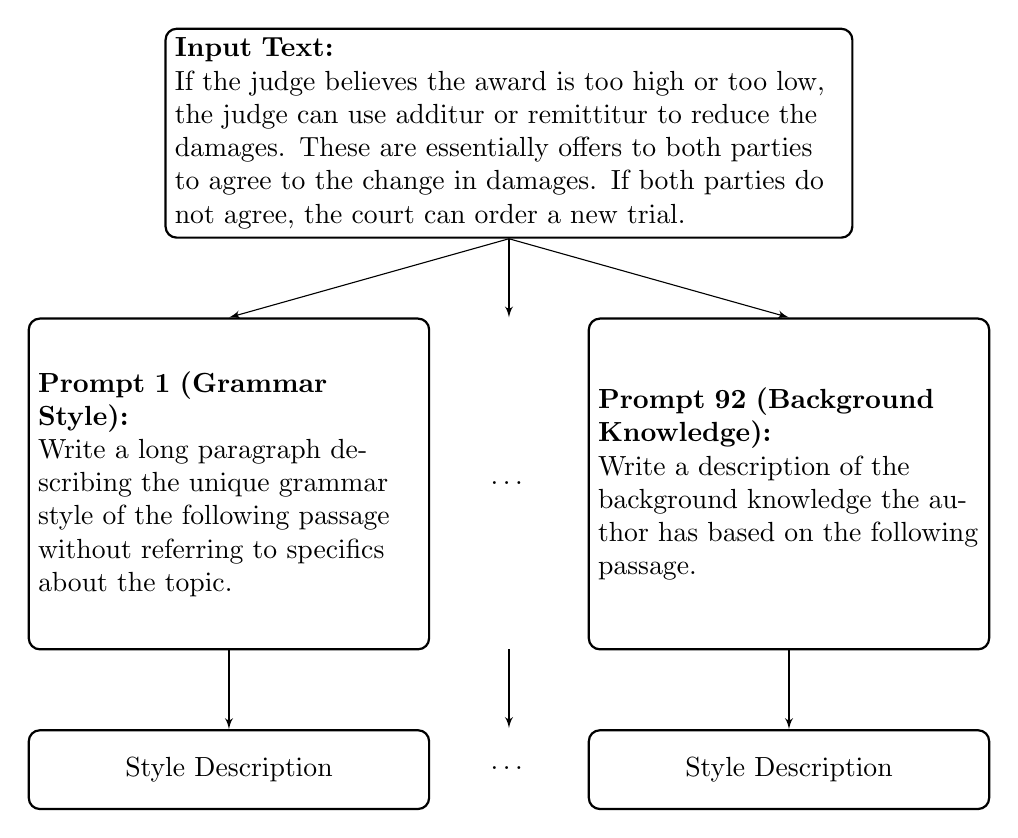
\begin{tikzpicture}
  [> = latex', auto,
    block/.style ={
        rectangle,
        draw=black,
        thick,
        % align=flush center,
        rounded corners,
        % minimum height=4em,
      },
  ]
  \node[block, text width=0.7\linewidth] (answer) {\textbf{Input Text:}\\If the judge believes the award is too high or too low, the judge can use additur or remittitur to reduce the damages. These are essentially offers to both parties to agree to the change in damages. If both parties do not agree, the court can order a new trial.};

  \node[block, minimum height=4.2cm, text width=0.4\linewidth, below left=of answer.south] (prompt1) {\textbf{Prompt 1 (Grammar Style):}\\Write a long paragraph describing the unique grammar style of the following passage without referring to specifics about the topic.};
  \node[align=flush center, minimum height=4.2cm, text width=0.2\linewidth, below=1cm of answer.south] (prompt2) {\ldots};
  \node[block, minimum height=4.2cm, text width=0.4\linewidth, below right=of answer.south] (prompt3) {\textbf{Prompt 92 (Background Knowledge):}\\Write a description of the background knowledge the author has based on the following passage.};

  \draw[->] (answer.south) -- (prompt1.north);
  \draw[->] (answer.south) -- (prompt2.north);
  \draw[->] (answer.south) -- (prompt3.north);

  \node[block, align=flush center, minimum height=1cm, text width=0.4\linewidth, below=1cm of prompt1] (description1) {Style Description};
  \node[align=flush center, minimum height=1cm, text width=0.2\linewidth, below=1cm of prompt2] (description2) {\ldots};
  \node[block, align=flush center, minimum height=1cm, text width=0.4\linewidth, below=1cm of prompt3] (description3) {Style Description};

  \draw[->] (prompt1.south) -- (description1.north);
  \draw[->] (prompt2.south) -- (description2.north);
  \draw[->] (prompt3.south) -- (description3.north);
\end{tikzpicture}

\end{frame}
\begin{frame}[shrink]
  \begin{tikzpicture}
  [> = latex', auto,
    block/.style ={
        rectangle,
        draw=black,
        thick,
        % align=flush center,
        rounded corners,
        % minimum height=4em
      },
  ]
  \node[block, align=flush center, minimum height=1cm, text width=0.4\linewidth, below=1cm of prompt1] (description1) {Style Description};
  \node[align=flush center, minimum height=1cm, text width=0.2\linewidth, below=1cm of prompt2] (description2) {\ldots};
  \node[block, align=flush center, minimum height=1cm, text width=0.4\linewidth, below=1cm of prompt3] (description3) {Style Description};

  \node[block, text width=0.95\linewidth, below=1cm of description2] (sentence_prompt) {\textbf{Prompt:}\\Rewrite this description as a long list of short sentences describing the author's writing style  where each sentence is in the format of \enquote{The author is X.} or \enquote{The author uses X.}.};

  \draw[->] (description1.south) -- ++(0,-1cm);
  \draw[->] (description2.south) -- ++(0,-1cm);
  \draw[->] (description3.south) -- ++(0,-1cm);

  \node[block, text width=0.95\linewidth, below=1cm of sentence_prompt] (attributes) {\textbf{Style Attributes:}\\
    % The author uses the passive voice. \\
    % The author uses active voice. \\
    % The author uses sentence fragments. \\
    % The author uses run-on sentences. \\
    % The author uses words related to visual perception. \\
    % The author uses words expressing wellness. \\
    % The author uses a neutral tone. \\
    The author uses words related to risk. \\
    The author uses words related to allure. \\
    The author uses words indicating poverty. \\
    The author uses words expressing needs. \\
    The author uses numbers. \\
    The author explains legal concepts. \\
    The author uses words indicating men. \\
    The author uses the word judge. \\
    \ldots
  };

  \draw[->] (sentence_prompt.south) -- +(0,-1cm);
  \draw[->] let \p1 = (sentence_prompt.south), \p2 = (description1) in (\x2,\y1) -- +(0,-1cm);
  \draw[->] let \p1 = (sentence_prompt.south), \p2 = (description3) in (\x2,\y1) -- +(0,-1cm);
\end{tikzpicture}

\end{frame}

\subsection{Clustering and Cluster Selection}
\begin{frame}{Clustering}
  \begin{itemize}
    \item the unique style sentences can be very similar as only exact equality is tested
          \begin{itemize}
            \item e.g. \enquote{The author uses long and complicated sentences} and \enquote{The author uses complicated and long sentences}
          \end{itemize}
    \item to improve further processing, the sentences are clustered
          \pause
          \begin{itemize}
            \item each sentence is in exactly one cluster
            \item all sentences in a cluster have a minimum cosine similarity of \num{0.85} to the center of the cluster
            \item the sentence closest to the center is the representation of the cluster
            \item style and knowledge sentences are clustered separately
          \end{itemize}
  \end{itemize}
\end{frame}

\begin{frame}{Resulting synthetic dataset}
  \begin{tabular}{lS}
    \toprule
                 & {Number of data points} \\ \midrule
    Answers      & 5500                    \\
    Prompts      & 92                      \\
    Descriptions & 506000                  \\
    Sentences    & \approx 3000000         \\
    Clusters     & \approx 1000000         \\ \bottomrule
  \end{tabular}
\end{frame}
\begin{frame}{Resulting synthetic dataset}{Current Data}
  \begin{tabular}{lS}
    \toprule
                 & {Number of data points} \\ \midrule
    Answers      & 1600                    \\
    Prompts      & 92                      \\
    Descriptions & 147200                  \\
    Sentences    & \approx 600000          \\
    Clusters     & \approx 290000          \\ \bottomrule
  \end{tabular}
\end{frame}

\begin{frame}{Cluster Selection}
  \begin{itemize}
    \item the final style vector will have 768 attributes
    \item the clusters are selected in multiple steps, where the most important criteria are as follows
          \begin{itemize}
            \item \num{84} attributes correspond to the 84 target prompts
            \item roughly \num{50} attributes are knowledge clusters
            \item style vector attributes must not have a cosine similarity higher than \num{0.7} to each other
            \item style vector attributes must not be used by more than \SI{60}{\percent} of the groups
          \end{itemize}
  \end{itemize}
\end{frame}


%%%%%%%%%%%%%%%%%%%%%%%%%%%%%%%%%%%%%%%%%%
\section{Custom Models}
\subsection{SFAM}
\begin{frame}{SFAM}{Style Feature Agreement Model\footauthorcite{patelLearningInterpretableStyle2023}}
  \begin{itemize}
    \item a fine-tuned DeBERTaV3 model
    \item gets a style sentence and a text as input and outputs an agreement score between \num{0} and \num{1}
    \item these agreement scores form the style vector
    \item SFAM is trained on the (unclustered) sentences
    \item Test Accuracy: \num{0.8964}, Test F1-score: \num{0.8992}
  \end{itemize}
\end{frame}

\begin{frame}{Most important attributes per group}{According to SFAM}
  \textbf{Lawyers}
  \begin{itemize}
    \item The author is discussing the judicial system.
    \item The author discusses laws and regulations.
    \item The author expresses skepticism towards the existing laws.
    \item The author uses words related to resolving disputes.
    \item The author references the Constitution.
    \item[+] The author has a background in law.
    \item[+] The author is familiar with the concept of a legislature.
  \end{itemize}
\end{frame}

\begin{frame}{Most important attributes per group}{According to SFAM}
  \textbf{Software Engineers}
  \begin{itemize}
    \item The author emphasizes the importance of flexibility in code.
    \item The author prioritizes clarity and simplicity in API design.
    \item The author uses code snippets.
    \item The author desires a solution that is easy to implement.
    \item The author advises against a particular approach.
    \item[+] The author is familiar with software system design and architecture concepts.
    \item[+] The author is skilled in Python programming.
  \end{itemize}
\end{frame}

\subsection{LISA}
\begin{frame}{LISA}{Linguistically Interpretable Style Attribute\footauthorcite{patelLearningInterpretableStyle2023}}
  \begin{itemize}
    \item a fine-tuned DeBERTaV3 model
    \item gets a text as input and outputs the style vector
    \item LISA is trained on style vectors that are produced by SFAM
    \item test performance
          \begin{itemize}
            \item MSE: \num{0.100}
            \item MAE: \num{0.220}
                  % \item Average Cosine Similarity: \num{0.701}
            \item Accuracy: \num{0.8318820529513888}
            \item F1: \num{0.7646265737452764}
          \end{itemize}
  \end{itemize}
\end{frame}

\subsection{Embedding Model}
\begin{frame}{Embedding Model}
  \begin{itemize}
    \item a simple model to convert the style vector to a style embedding
    \item different style vectors can not be meaningfully compared
    \item the model is trained with a triplet loss with a contrastive objective
    \item training data are style vectors for the different groups
    \item Test Accuracy on SFAM embeddings: \num{0.8417}
  \end{itemize}
\end{frame}

\begin{frame}[plain]
  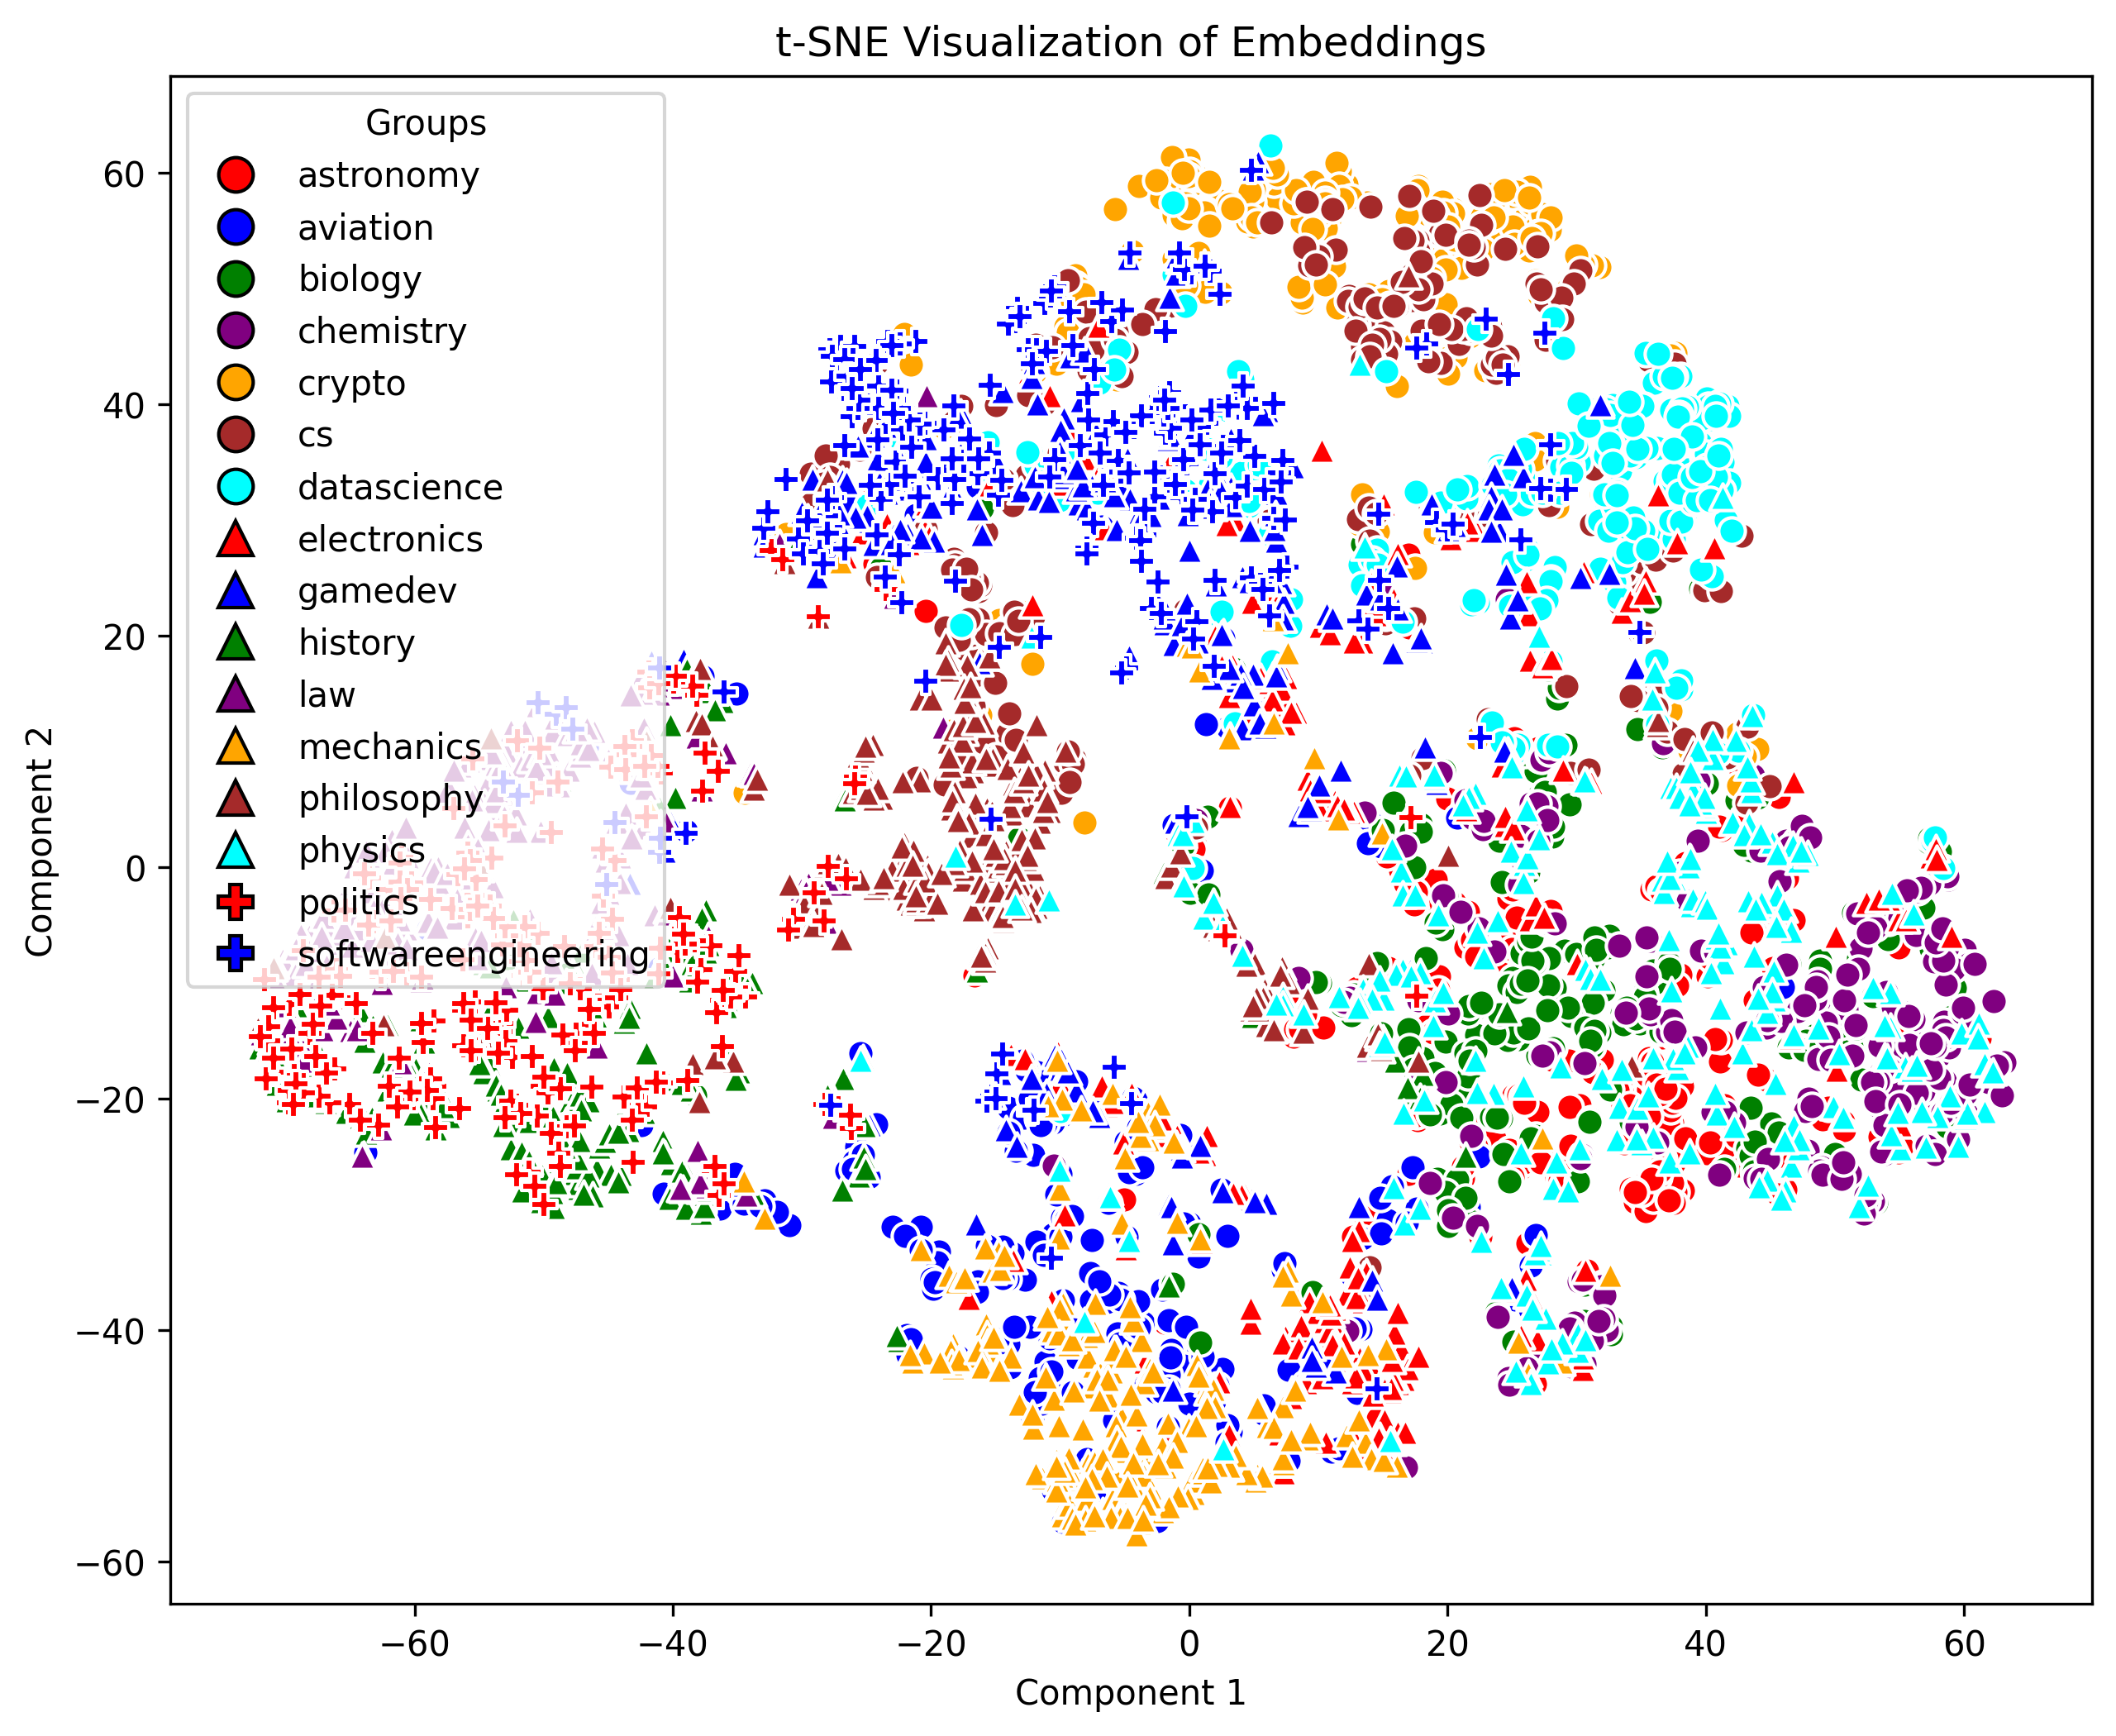
\includegraphics[width=\linewidth]{img/t-SNE-embedding.png}
\end{frame}


%%%%%%%%%%%%%%%%%%%%%%%%%%%%%%%%%%%%%%%%%%
\section{Steering Text Generation}
\subsection{Steering with Prompt Engineering}
\begin{frame}{Steering with Prompt Engineering}
  \begin{description}
    \item[Prompt Group] ~\linebreak
          The LLM is instructed in the system prompt to write for a group of <group>.
    \item[Prompt Attribute] ~\linebreak
          The LLM is instructed to write in a specific style. The 5 most important style attributes and the 2 most important knowledge attributes are used.
    \item[Prompt Group Attribute] ~\linebreak
          A combination of both.
  \end{description}
\end{frame}

\begin{frame}{Results I}
  \begin{itemize}
    \item performance of different steering methods, averaged over all groups
          \begin{itemize}
            \item euclidean distance: how big was the steering effect
            \item cosine similarity: was the steering in the correct direction
                  \begin{itemize}
                    \item measurement between the steering difference and the median embedding of the group
                  \end{itemize}
          \end{itemize}
  \end{itemize}
  \begin{tabular}{lSS}
    \toprule
    {Steering\ Type}         & {Euclidean\ Distance}                              & {Cosine\ Similarity}                                \\
    \midrule
    Prompt\ Group            & 1.3857046365737915                                 & 0.2616930603981018                                  \\
    Prompt\ Attribute        & 1.6388777494430542                                 & 0.38969555497169495                                 \\
    Prompt\ Group\ Attribute & \cellcolor[gray]{0.8} \bfseries 1.9113191366195679 & \cellcolor[gray]{0.8} \bfseries 0.42248931527137756 \\
    \bottomrule
  \end{tabular}
\end{frame}

\begin{frame}{Results II}
  \begin{itemize}
    \item performance for different groups, averaged over all steering methods
    \item only the 4 best and 4 worst performing groups are shown
  \end{itemize}
  \begin{tabular}{lSS}
    \toprule
    {Group}              & {Euclidean\ Distance}                              & {Cosine\ Similarity}                               \\
    \midrule
    Astronomers          & 1.5674035549163818                                 & 0.4043354094028473                                 \\
    Computer Scientists  & 1.3228683471679688                                 & 0.2554630935192108                                 \\
    Electrical Engineers & 1.2279574871063232                                 & 0.12286949157714844                                \\
    Game Developers      & 1.3090592622756958                                 & -0.017543332651257515                              \\
    Lawyers              & \cellcolor[gray]{0.8} \bfseries 2.6319475173950195 & \cellcolor[gray]{0.8} \bfseries 0.7551590204238892 \\
    Philosophers         & 2.3561315536499023                                 & 0.7398480176925659                                 \\
    Politicians          & 2.535012722015381                                  & 0.702243983745575                                  \\
    Software Engineers   & 1.3615081310272217                                 & 0.1768019199371338                                 \\
    \bottomrule
  \end{tabular}
\end{frame}

% \begin{frame}{Results III}
%   \begin{itemize}
%     \item performance for different groups for the prompt group attribute method
%     \item only the 4 best and 4 worst performing groups are shown
%   \end{itemize}
%   \begin{tabular}{lSS}
%     \toprule
%     {Group}              & {Euclidean\ Distance}                              & {Cosine\ Similarity}                               \\
%     \midrule
%     Biologists           & 1.5506118535995483                                 & 0.33786728978157043                                \\
%     Data Scientists      & 2.1414427757263184                                 & 0.49583321809768677                                \\
%     Electrical Engineers & 1.334580421447754                                  & 0.03393082693219185                                \\
%     Game Developers      & 1.4480421543121338                                 & 0.044030994176864624                               \\
%     Lawyers              & 3.108609199523926                                  & \cellcolor[gray]{0.8} \bfseries 0.8223204016685486 \\
%     Philosophers         & 2.6420016288757324                                 & 0.7476155757904053                                 \\
%     Politicians          & \cellcolor[gray]{0.8} \bfseries 3.1334586143493652 & 0.7666002511978149                                 \\
%     Software Engineers   & 1.611264705657959                                  & 0.2527718245983124                                 \\
%     \bottomrule
%   \end{tabular}
% \end{frame}

\begin{frame}{System Prompt Game Developers}{Prompt Group Attribute Steering}
  \justifying
  You are an author that writes a helpful explanation for a group of game developers.

  You emphasize the importance of flexibility in code. You desire a solution that is easy to implement. You use code snippets. You discuss a visual perception concept related to movement. You advise against a particular approach.

  You understand geometric concepts. You present two possible approaches.
\end{frame}

\begin{frame}{System Prompt Lawyers}{Prompt Group Attribute Steering}
  \justifying
  You are an author that writes a helpful explanation for a group of lawyers.

  You are discussing the judicial system. You discuss laws and regulations. You express skepticism towards the existing laws. You use words related to resolving disputes. You reference the Constitution.

  You have a background in law. You are familiar with the concept of a legislature.
\end{frame}

% TODO: steered generations on backup slides


\subsection{Activation Steering}
\begin{frame}{Activation Steering}{Concept}
  \begin{itemize}
    \item idea: steer the model by manipulating its activation space\footauthorcite{turnerActivationAdditionSteering2024,rimsky-etal-2024-steering}
    \item previous work has shown that real-world concepts are represented as direction in the activation space
    \item the activation vectors are extracted for all layers of the model in a single forward pass
    \item during steering, the activation vector is added to the layer it was taken from
  \end{itemize}
\end{frame}

\begin{frame}{Activation steering}{Process}
  \begin{itemize}
    \item for each style vector attribute, the activation vector at every layer of the large language model is extracted from one forward pass
    \item the steering vectors for a group are constructed by weighing the steering vectors for all style vector attributes by the softmax of the style vector of the group
    \item in the experiments, the activation steering will be combined with prompt steering methods
    \item this part is not yet implemented by me
  \end{itemize}
\end{frame}

%%%%%%%%%%%%%%%%%%%%%%%%%%%%%%%%%%%%%%%%%%
\section{Conclusion}
\begin{frame}{Conclusion}
  \begin{itemize}
    \item the presented method is one automatic process from input data to a model with steering capabilities
    \item the models show promising results
  \end{itemize}
\end{frame}


%%%%%%%%%%%%%%%%%%%%%%%%%%%%%%%%%%%%%%%%%%
\begin{frame}[c]
  \centering \Large
  Thank you for your attention

  \vspace{0.5em} \large
  Are there any questions?
\end{frame}

%%%%%%%%%%%%%%%%%%%%%%%%%%%%%%%%%%%%%%%%%%
\section*{References}
\begin{frame}[allowframebreaks]{References}
  \printbibliography
\end{frame}


%%%%%%%%%%%%%%%%%%%%%%%%%%%%%%%%%%%%%%%%%%
\section*{Backup Slides}
\begin{frame}[plain]
  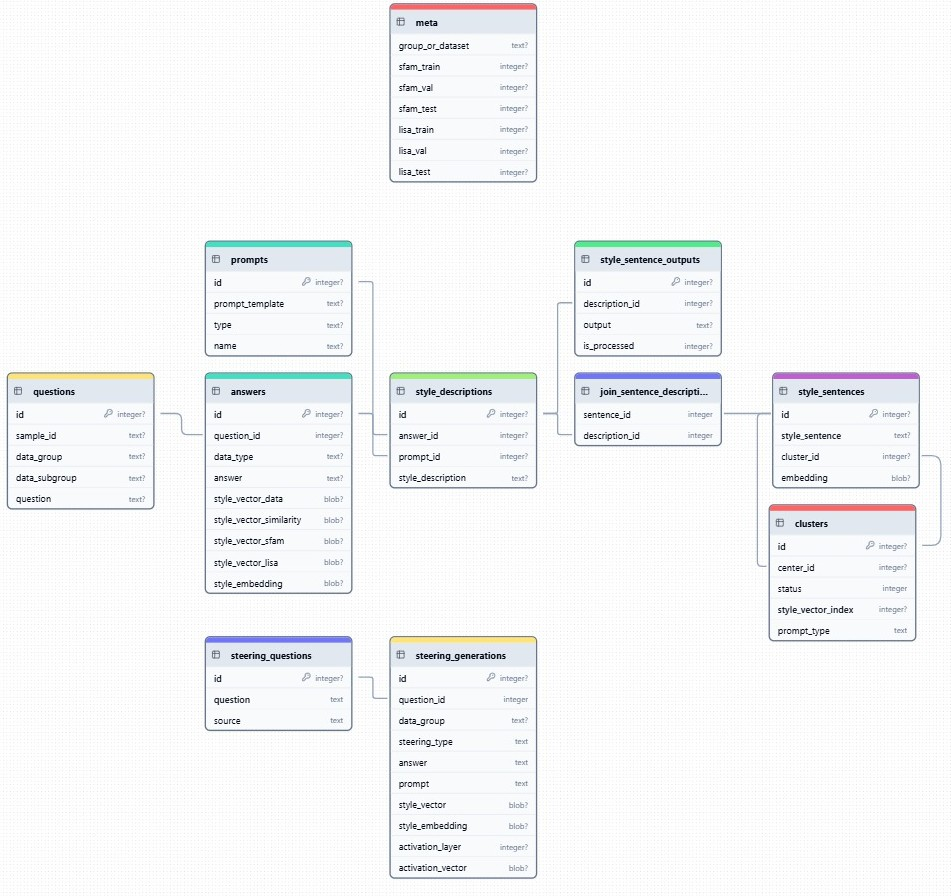
\includegraphics[width=\linewidth]{img/sqlite-db.jpeg}
\end{frame}


\end{document}
